\scanpage{151}
\mspage{75}

Prouvons a). Soit \(\Gamma'\subset\mathcal E\)
\inserted{section partielle sur \(\Gamma_x\)}
déduite de \(x\in U^!\).
Soit \(\Gamma''\supset\Gamma'_x\) un autre \unsure{ss-groupe|sous-groupe}
\inserted{soit \(\unsure{\Gamma_1}\supset\Gamma_x\) son image \unsure{ds|de} \(\Gamma\)}
tel que \(\Gamma''\cap\pi=(1)\) i.e. \(\Gamma''\hookrightarrow\Gamma\)
\inserted{\illegible{1}}.
Par le th. précédent, il est défini par un unique
\unsure{\(y\in U^{\Gamma_1}\)|\(y\in U^{\Gamma''_*}\)},
et il est clair que cet \(y\) ne change pas si on remplace l'action de
\(\unsure{\Gamma_1}\) sur \(U\) par l'action d'un groupe plus petit
\(\ne(1)\) (et la section induite) tel \(\Gamma_x\),
donc \(\unsure{\Gamma_1}\) \deleted{\illegible{1}} fixe \(x\) donc
(par définition de \(\Gamma_x\)) \(\Gamma_1=\Gamma_x\) donc
\(\Gamma''=\Gamma'\), \deleted{\unsure{cqfd.}}

\deleted{\unsure{L'injec}}\inserted{b)}
Soient \(x,y\) donnant \(\overline{\mathrm m}\) image
\([\Gamma']\ [\Gamma'']\), donc \(\Gamma_x=\Gamma_y\), soit \(\Gamma_1\),
et appliquant le \unsure{thm} à \(\Gamma_1\) opérant sur \(U\),
on trouve \(x=y\).
Soit d'autre part \(\Gamma'_0\) une section partielle \(\ne1\) maximale,
\(\Gamma_0\subset\Gamma\) son image,
par le th. \inserted{appliqué à l'action de \(\Gamma_0\) sur \(U\),}
\(\exists x\in U\) \deleted{\unsure{fixe}} tel que
\(x\in U^{\Gamma'_0}\) i.e. \(\Gamma'_0\subset\Gamma_x\),
et que \([\Gamma'_0]\) soit défini par \(x\),
mais si \([\Gamma']\) est défini par \(x\) pour l'action de
\(\Gamma_x\) tt entier, on aura \([\Gamma'_0]\subset[\Gamma']\),
donc par le car. maximal de \([\Gamma'_0]\), on aura
\([\Gamma'_0]=[\Gamma']\), ce \deleted{\illegible{1}} qui prouve b).
D'autre part c) est clair.

\margin{150}

\scanpage{152}

Revenons maintenant au cas où \(U=X\setminus S\), \(X\) surface
\(T\)-orientée compacte et \(S\) partie
finie, cas anabélien --- donc on a une description
\inserted{``plt} fidèle'' de \(U\) par un \(\pi\) avec
structure à lacets, et on voudrait se convaincre
que \deleted{\illegible{2}} l'op. \inserted{extérieure} de \(\Gamma\)
sur \(\pi\), quand \(\Gamma\) conserve l'orientation (pour simplifier)
également \unsure{suffit} pour décrire pleinement l'objet
\((U,\Gamma)\) dans le catégorie isotopique qui convient.
\margin{il faudrait revenir sur le cas général pour \unsure{la suite}\ldots}

On récupère déjà une description de \(\unsure{U^!}\) en termes de
l'action de \(\pi\), soit \(J\) \inserted{\((\simeq U^!)\)},
l'ens des classes de \(\pi\)-conjugaison
\deleted{de plus pour tt \(x\)}
de sections partielles \inserted{\(\ne1\)} maximales de
\(\mathcal E\) sur \(\Gamma\),
Pour tt \(j\in J\), \(j\) est un \inserted{\(\pi\)-}torseur
comme
classe de \inserted{\(\pi\)-}conjugaison de sections
[que ce soit un \(\pi\)-torseur résulte de
\(\pi^{\Gamma'}=(1)\), a priori
\deleted{\unsure{c'est un \(\pi/\pi^{\Gamma'}\)-torseur}}
\inserted{\unsure{le stabilisateur|les stabilisateurs} de \(\Gamma'\)}
est \(\pi^{\Gamma'}\) justement]
En fait,

\margin{151}

\scanpage{153}
\mspage{76}

l'ensemble de \unsure{ttes} ces \deleted{\unsure{classes}} sections
partielles maximales est de façon naturelle un \(\mathcal E\)-ensemble
(par conjugaison) \deleted{\unsure{et}} sur lequel \(\pi\) opère librement, et cet
\(\mathcal E\)-ensemble s'identifie canoniquement à
\(\widetilde U|U^!=\widetilde U^!\), pour la structure de
\(\mathcal E\)-ensembles.

Soit \(S'=S\cup U^!\), donc \(U'=X\setminus S'\),
il s'impose d'essayer de reconstituer
(en termes de l'extension \(\mathcal E\) de \(\Gamma\) par le groupe à
lacets \(\pi\)) le groupe \inserted{extérieur} à lacets correspondant
à \(\unsure{X'},S'\) i.e. à \(U'\), et l'\deleted{extension}
\inserted{action extérieure} de \(\Gamma\) sur celui-ci.
\deleted{\unsure{On espère trouver un} \illegible{5}}
\deleted{\(\unsure{=}\) \illegible{5} \unsure{évident}}

Mais il faudrait d'abord s'assurer du caractère intrinsèque de la
définition de \(J\) \unsure{\((\simeq U^!)\)|\((\simeq\widetilde U^!)\)}
\inserted{comme \(\Gamma\)-ensemble,}
en termes du \deleted{l'action} \deleted{du}
groupe extérieur \(\pi\), et de l'action
\deleted{de \(\unsure{\Gamma}\)} extérieure de \(\Gamma\) dessus.

\margin{152}

\scanpage{154}

Ceci est assez évident d'ailleurs
(en termes \inserted{justement} des classes de
\inserted{\(\pi\)-}conjugaison de relèvements partiels de
\(\unsure{\Gamma\to\operatorname{Autext}(\pi)}\) vers
\(\operatorname{Aut}(\pi)\)), on aimerait cependant aussi une
description intrinsèque de \(\widetilde U|U^!\),
\unsure{en|ou} un paradigme pour l'application de
\(\Gamma\)-espaces \(\unsure{U^!\longrightarrow U}\)
on doit donc décrire un morphisme de topos avec op. de \(\Gamma\) dessus
\diagram{\begin{tikzcd}[ampersand replacement=\&]
B_J \arrow[r,"\unsure{\rho}"] \& B_{\unsure{\mathcal E}}
\end{tikzcd}}
qui correspond donc à un \deleted{\unsure{morph}} foncteur
``image inverse'' \(\unsure{\rho^*|?^*}\)
(compatible avec action de \(\Gamma\))
\deleted{\illegible{1}}
\diagram{\begin{tikzcd}[ampersand replacement=\&,row sep=2.5em,column sep=4em]
B_{\unsure{\mathcal E}} \arrow[r] \arrow[d,phantom,"\simeq"{description,rotate=90}] \& B_J \arrow[d,phantom,"\simeq"{description,rotate=90}] \\
\pi\text{-Ens} \& \mathrm{Ens.}\ \text{sur }J
\end{tikzcd}}

Ce \deleted{\unsure{qui}} n'est autre que le produit contracté sur
\(\pi\) avec l'ens des sections partielles \(\ne1\) maximales de
\(\mathcal E\) sur \(\Gamma\)

\margin{153}

\scanpage{155}
\mspage{77}

Revenons à l'extension \(\mathcal E\) de \(\Gamma\) par \(\pi\)
\deleted{\unsure{avec op. fidèle de \(\Gamma\)}}
provenant d'une situation géométrique
(laquelle extension, dans le cas anabélien, est définie déjà en termes
d'une op. extérieure de \(\Gamma\) sur \(\pi\))
on sait que celle-ci satisfait des conditions supplémentaires
draconiennes !
\inserted{\deleted{\unsure{pour}} (Pour les formuler, on va supposer l'action de
\(\Gamma\) fidèle) :}
tt sous-groupe \(\Gamma'\subset\mathcal E\) tel que
\(\Gamma'\cap\pi=(e)\) (``section partielle'') est
\inserted{cyclique (si \(\Gamma'=\Gamma'{}^0\)) ou}
\deleted{\illegible{1}} diédral,
\inserted{(si \(\Gamma'\ne\Gamma'{}^0\))}
et l'ensemble des classes de \(\pi\)-conjugaison de tels ss-groupes
est fini.
Tout sous-groupe section \(\Gamma'\ne1\) est contenu dans un unique
ss groupe \inserted{section} \uline{maximal}.
\margin{\unsure{bon|donc}
\figure{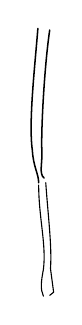
\begin{tikzpicture}[x=1mm,y=1mm,baseline=(current bounding box.center),line cap=round,line join=round]
\draw[line width=0.55pt] (0,34) .. controls (-0.4,29) and (-1.2,22) .. (-0.7,18.5) .. controls (-0.6,16.5) and (0.1,15.5) .. (0.1,14.4);
\draw[line width=0.40pt] (0.1,14.1) .. controls (0.1,10) and (1.1,6.5) .. (0.7,3.4) .. controls (0.4,1.8) and (0.3,0.9) .. (0.7,0);
\draw[line width=0.55pt] (1.5,33.8) .. controls (0.8,29) and (0.4,21) .. (0.5,18.5) .. controls (0.6,16.9) and (0.1,15.5) .. (0.8,15.0);
\draw[line width=0.40pt] (1.0,14.4) .. controls (1.3,10.1) and (1.8,6.3) .. (1.6,3.5) -- (2.0,0.5) -- (1.5,0.1);
\end{tikzpicture}}}

(On l'a établi tt au moins dans le cas
\(\Gamma=\Gamma^0\), il faudrait revenir sur le cas général,
je pense que ça reste vrai tel quel, à vérifier\ldots)
\margin{\figure{[Un trait vertical à gauche des deux lignes
« je pense \ldots{} vérifier\ldots) ».]}}
De plus, on vit apparaître une \uuline{structure supplémentaire}
sur le groupe \(\mathcal E\)
[qui dans le cas anabélien s'identifie à un sous-groupe de
\(\operatorname{Aut}(\pi)\)], à savoir une application
\[
\mu_{\mathcal E}:
\text{éléments }\inserted{u}\text{ d'ordre fini de }\mathcal E
\longrightarrow T\otimes\mathbb Q/\mathbb Z,
\]
\unsure{obtenue} en notant que si \(u\in\mathcal E\) est d'ordre fini
\(n\), \unsure{d'où} \(\mathbb Z/n\mathbb Z\lhook\joinrel\xrightarrow[i]{}
\mathcal E\), \unsure{on a|i.e.} \(\operatorname{Im}i\cap\pi=(1)\)
(\(\pi\) n'a pas d'éléments de torsion), donc
\(\mathbb Z/n\mathbb Z\hookrightarrow\Gamma\), \unsure{d'où|d'un} sous-groupe
\(\Gamma_1\subset\Gamma\) (i.e. l'image de
\margin{\uline{NB} Pour un \(u\) d'ordre fini de \(\mathcal E\),
on doit \unsure{savoir|avoir}, si \(u\notin\mathcal E^0\),
que \(u\) \unsure{est} d'ordre \(2\) exactement,
\illegible{5} pour \unsure{définir} \(\mu(u)\)!}

\margin{154}

\scanpage{156}

\(\unsure{u}\) dans \(\Gamma\) a \(\overline{\mathrm m}\) ordre \(n\)),
et le relèvement \(\Gamma_1\hookrightarrow\mathcal E\) définit un
\(x\in U^{\Gamma_1}\), \deleted{tel que} et \(u_1\) opérant sur \(U\)
en laissant fixe \(x\) correspond donc au voisinage de \(x\) à un
``multiplicateur'', qui (pour une orientation locale choisie) est une
racine primitive \unsure{\(n\).ième} de \(1\) i.e. un élément de
\(\mathbb Z/n\mathbb Z\), et qui pour orientation changeante
s'interprète intrinsèquement comme élément de
\(T\otimes\mathbb Z/n\mathbb Z
\subset T\otimes\mathbb Q/\mathbb Z\).

L'application \(\mu\) satisfait les conditions évidentes
\[
\begin{gathered}
\left\{
\begin{aligned}
\mu(\alpha u\alpha^{-1})&=\mu(u) &&\text{si }\alpha\in\pi\\
\mu(u^n)&=n\mu(u) &&\text{si }n\in\mathbb Z
\end{aligned}
\right.\\
\text{ordre }\mu(u)=\text{ordre de }u
\end{gathered}
\]
J'ignore si cette application \(\mu\) \deleted{est}
\inserted{peut se} définir intrinsèquement en termes de l'extension
\(\mathcal E\), ou si au contraire il peut exister deux extensions
\deleted{\unsure{iso}} \(\mathcal E,\mathcal E'\) de \(\Gamma\) par \(\pi\),
définies par des situations géométriques, de \(\Gamma\) opérant sur
\(U\) resp. \(U'\), et un isom. d'extensions
\(\mathcal E\longrightarrow\mathcal E'\) qui ne soit compatible avec
les fonctions \(\mu,\mu'\).
Le cas non trivial le plus simple à regarder est le cas

\margin{155}

\scanpage{157}
\mspage{78}

abélien (où \(\pi\simeq\mathbb Z\)
\inserted{\deleted{\illegible{1}} \((\operatorname{card}I=2)\)}
ou \(\pi\simeq\mathbb Z^2\) (\deleted{\unsure{card}} \(I=\varnothing\))),
Dans le \inserted{premier} cas
\deleted{d'une extension} \(\pi\simeq\mathbb Z\), \unsure{on|\deleted{les}}
\inserted{doit avoir (pour avoir une action fidèle de
\(\Gamma=\Gamma^0\))}
\deleted{extensions \illegible{1}}
\(\Gamma^0\) cyclique, \(\mathcal E\simeq\mathbb Z\),
il n'y a pas d'élément d'ordre fini dans \(\mathcal E\) sauf
\(\unsure{1|e}\), donc la question ne se pose pas.
Le cas \(\pi\simeq\mathbb Z^2\) est plus intéressant,
\deleted{\unsure{et peut se reformuler}}

Si \(\pi\) est un \(\mathbb Z\)-module libre de
\deleted{\unsure{t.f.}}\inserted{\unsure{rg \(n\)}}, on a une suite exacte
\diagram{
\begin{tikzcd}[column sep=small,row sep=small]
0 \arrow[r] & \pi \arrow[r] & \pi\otimes_{\mathbb Z}\mathbb R
\arrow[r] & X_0(\pi) \arrow[r] \arrow[d,dash] & 0\\
& & & \substack{\text{Tore de dim}\\ n\text{ associé à }\pi} &
\end{tikzcd}
}
et si \(\Gamma\) opère sur \(\pi\), la suite exacte de cohomologie
(compte tenu de \(H^i(\Gamma,\pi\otimes_{\mathbb Z}\mathbb R)=0\)
pour \(i>0\)) donne
\diagram{
\begin{tikzcd}[column sep=large,row sep=small]
H^2(\Gamma,\pi) & H^1(\Gamma,X_0(\pi)) \arrow[l,"\sim" {anchor=south}]\\
\substack{\text{\unsure{classe d'extension|classes d'extensions}}\\
\text{de }\Gamma\text{ par }\pi}
&
\substack{\text{classes de}\\X_0(\pi)\text{ torseurs,}\\
\text{avec op. de }\Gamma\text{ dessus}\\
\text{compatible avec son}\\\text{action sur }X_0(\pi)}
\end{tikzcd}
}

donc la donnée d'une extension \(\mathcal E\) de \(\Gamma\) par \(\pi\)
revient essentiellement à celle d'un
\unsure{\(\Gamma\)-\(X_0(\pi)\)-torseur} \(X\)
(\(n\)-tore inhomogène sur lequel \(\Gamma\) opère --- donc il opère
sur son groupe des translations \(X_0\), donc sur
\(\pi=\pi_1(X_0,0)\)\ldots).
S'il était vrai \inserted{pour \(n=2\)} que tte opération

\margin{156}

\scanpage{158}

de \(\Gamma\) sur une surface torique \((\simeq S^1\times S^1)\)
est isomorphe à une telle action standard, alors le caractère
intrinsèque de l'application \(\mu\) dans ce cas serait établi
--- ce qui ne \unsure{rendrait} pas inintéressant pour autant le calcul
de \(\mu\), qui prend ses valeurs dans
\(T\otimes\mathbb Q/\mathbb Z\), où ici
\[
T\simeq\bigwedge\nolimits_{\mathbb Z}^{2}\pi
\quad
(\text{\unsure{dual|dim.\ 2} de }H^2(\pi,\mathbb Z)\simeq
\bigwedge\nolimits^{2}
\underbrace{H^1(\pi,\mathbb Z)}_{
\substack{\unsure{\downarrow|\simeq}\\ \pi^\vee}}).
\]

La question revient à celle-ci : On a une extension \uline{scindée}
d'un \deleted{\unsure{groupe}}\inserted{\unsure{groupe}} cyclique
\(\mathbb Z/n\mathbb Z\) de générateur \(u\) par \(\pi\)
--- décrite donc entièrement par un autom.
\deleted{d'ordre} \(\unsure{\theta}\) de \(\pi\) tel que
\(\theta^n=\operatorname{id}_\pi\)), décrire \unsure{en} termes de
ceci un élément de \(T\otimes\mathbb Q/\mathbb Z\).

Réponse : la situation géométrique \unsure{standard|st. dont}
correspond à \(X=X_0(\pi)\), avec \(0\) comme pt fixe sous \(\Gamma\).
Si \(u\) renverse l'orientation, il est d'ordre \unsure{\(1\) ou|i.e.} \(2\),
il n'y a pas de Pb, sinon c'est \deleted{dans} en
\(\pi\otimes_{\mathbb Z}\mathbb R\) une rotation autour de \(0\)
(d'ordre \(2,3,4\) ou \(6\)) qui se repère bien par un élément
de \deleted{\illegible{1}} \(T\otimes\mathbb Z/\nu\mathbb Z\)
(si \(\nu\) est \unsure{d'ordre|l'ordre}).
C'est aussi (si on identifie
\(T\otimes\mathbb Z/\nu\mathbb Z\) à
\(\mu_\nu(\mathbb C^*)\), en supposant
\(T\simeq\mathbb Z\) donné
i.e. \(\pi\) orienté i.e. \(X_0(\pi)=\unsure{X}\)
orienté) \uline{une} des deux

\margin{157}

\scanpage{159}
\mspage{79}

valeurs propres de \(u\otimes_{\mathbb Z}\mathbb C\)
(autom du vectoriel sur \(\mathbb C\) de dim \(2\)
\(\pi\otimes_{\mathbb Z}\mathbb C\)).

Ceci nous montre, dans le cas de la géom Alg sur corps alg clos
\(\Omega\), que si \(X=X_0\) est une courbe elliptique
\(u\) un autom d'ordre fini, on a comme description
paradigmatique non \uline{seult}
\(\pi=\pi_1(X,0)\)
\inserted{(\(\widehat{\mathbb Z}\)-module libre de rg \(2\)),}
(et l'action de \(u\) sur \(\pi\)), mais comme structure
\uline{supplémentaire} l'une des deux solutions \uline{dans \(\Omega\)}
de l'équation caractéristique de \(u\) (à coefficients entiers)
\[
T^2+aT+b=0
\qquad (a=-\operatorname{Tr}u,\ b=\unsure{\det u}).
\]

Il est clair que cette structure supplémentaire ne peut se déduire
de la seule connaissance de l'action de \(u\) sur \(\pi\).
\margin{\figure{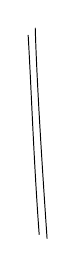
\begin{tikzpicture}[x=1mm,y=1mm,baseline=(current bounding box.center),line cap=round]
\draw[line width=0.35pt] (0,25.8) .. controls (0.4,19) and (0.7,10) .. (1.4,0.5);
\draw[line width=0.35pt] (0.9,26.7) .. controls (1.1,19.7) and (1.8,8.8) .. (2.4,0);
\end{tikzpicture}}
pour \(\unsure{\Omega}=\mathbb C\)
\illegible{2} \unsure{revient à}
\illegible{1} \uline{\unsure{orientation|orientations}} de
\illegible{1}}
Mais il reste la question si cette \deleted{\unsure{dernière}}
\inserted{\unsure{\(\mu(u)\in\mu_n^*(\Omega)\)}}
peut se déduire de la connaissance au moins de l'action
\inserted{extérieure} de \(u\) sur le groupe
``avec \(1\) lacet'' correspondant à la situation géométrique
--- i.e. un autom \inserted{ext.}
\deleted{\illegible{2}} d'ordre \(n\) \unsure{d'} un tel groupe
(ou si là encore il faut la considérer décidément comme une donnée
supplémentaire).
\margin{oui, il le peut, grâce à la considération des
``sous-groupes \illegible{2} de \(\mathcal E\)''
\illegible{2} qui définissent des extensions
\diagram{\begin{tikzcd}[ampersand replacement=\&,row sep=2.5em,column sep=2em]
\unsure{1} \arrow[r] \& T \arrow[r] \arrow[dr,dotted,no head,"\unsure{n_i\,\mathrm{id}_T}"'] \& \mathcal E_i \arrow[r] \arrow[d,phantom,"\simeq"{description,rotate=90}] \& \Gamma_i \arrow[r] \& 1 \\
\& \& T \& \&
\end{tikzcd}}
d'où \(\unsure{\Gamma_i\simeq T/n_iT}\)
\illegible{2}}
Mais s'il en était bien ainsi, cela impliquerait d'autre part que la
construction de \unsure{\(u\in\) groupe|ces groupes} à

\margin{158}

\scanpage{160}

(1) lacet(s), avec l'op. de \(\Gamma\) dessus, ne peut se faire non
plus à l'aide de la seule \deleted{\illegible{2}}
connaissance de l'action de \(\Gamma\) (\(=\mathbb Z/n\mathbb Z\))
sur \(\pi\).
C'est cette question de ``forage de trous'' qu'il faut donc en fin de
compte, à la fin des fins, attaquer !

Quant à la question de savoir si
\deleted{\illegible{1}}\inserted{dans}
\deleted{\illegible{1}} le \uline{cas anabélien},
l'application
\[
\mu:\underbrace{{}_\infty\mathcal E}_{
\substack{\text{\unsure{ens des}}\\
\text{\unsure{élémts}}\\
\text{d'ordre fini de }\mathcal E}}
\longrightarrow T\otimes\mathbb Q/\mathbb Z)
\]
est déductible de l'action de \(\Gamma\) sur \(\pi\)
[si elle est fidèle, \(\mathcal E\) s'identifie donc à un ss-groupe
de \(\operatorname{Autext}_{\unsure{\ell|l}}(\pi)\)
et on peut se demander si \(\mu\) n'est pas
\inserted{alors} définissable sur cet tt entier],
ou \unsure{c'est|si c'est} une donnée supplémentaire dont il faut disposer pour
reconstituer la situation géom. --- la question reste entière.
\margin{cela semble bien \unsure{ainsi}, compte tenu
\illegible{1} que pour \(\Gamma\) \uline{résoluble},
\illegible{3}, on sait \illegible{1}
que tte action \deleted{\illegible{1}} de \(\Gamma\) sur \(\pi\)
\illegible{3} \unsure{réaliser géométriquement}}

\textcircled{16}\quad
\uuline{Bouchage et forage de trous:}
\uline{Préliminaires} \unsure{toposiques} généraux

Considérons une situation
\diagram{
\begin{tikzcd}
B_{D^*} \arrow[r] & B_U
\end{tikzcd}
}
(de topos multigaloisiens)
\margin{NB. une telle situation
\inserted{toposique \unsure{décrit}} \(2\)-fidlt les situations topologiques \((X,S)\),
ou \(U\), pourvu qu'aucune composante irréductible de \(U\)
ne soit \(\simeq S^2\) ---}

\margin{159}
